%!TEX encoding = UTF-8 Unicode
\documentclass[11pt, a4paper, twoside]{article}   	% use "amsart" instead of "article" for AMSLaTeX format

\usepackage{geometry}                		% See geometry.pdf to learn the layout options. There are lots.
\usepackage{listings}				% For Source Code displaying
\usepackage[german]{babel}			% this end the next are needed for german umlaute
\usepackage[utf8]{inputenc}
\usepackage{color}
\usepackage{graphicx}
\usepackage{titlesec}
\usepackage{fancyhdr}
\usepackage{lastpage}
\usepackage{hyperref}
% http://www.artofproblemsolving.com/wiki/index.php/LaTeX:Symbols#Operators
% =============================================
% Layout & Colors
% =============================================
\geometry{
   a4paper,
   total={210mm,297mm},
   left=20mm,
   right=20mm,
   top=20mm,
   bottom=30mm
 }	

\definecolor{myred}{rgb}{0.8,0,0}
\definecolor{mygreen}{rgb}{0,0.6,0}
\definecolor{mygray}{rgb}{0.5,0.5,0.5}
\definecolor{mymauve}{rgb}{0.58,0,0.82}

\setcounter{secnumdepth}{4}


% the default java directory structure and the main packages
\newcommand{\srcDir}{../src/main/java}
\newcommand{\srcTestDir}{../src/test/java}
\newcommand{\mainPackage}{\srcDir/at/fhooe/swe4/lab3}
\newcommand{\mainTestPackage}{\srcTestDir/at/fhooe/swe4/lab3/test}
\newcommand{\imagesDir}{images}
% the default subsection headers
\newcommand{\ideaSection}{Lösungsidee}
\newcommand{\sourceSection}{Source-Code}
\newcommand{\testSection}{Tests}


% =============================================
% Code Settings
% =============================================
\lstdefinestyle{sourceFileStyle}{ %
  basicstyle=\tiny,        % the size of the fonts that are used for the code
  breakatwhitespace=false,         % sets if automatic breaks should only happen at whitespace
  breaklines=true,                 % sets automatic line breaking
  captionpos=t,                    % sets the caption-position to top
  commentstyle=\color{mygreen},    % comment style
  frame=single,                    % adds a frame around the code
  keepspaces=true,                 % keeps spaces in text, useful for keeping indentation of code (possibly needs columns=flexible)
  keywordstyle=\color{blue},       % keyword style
  language=JAVA, 
  numbers=left,                    % where to put the line-numbers; possible values are (none, left, right)
  numbersep=5pt,                   % how far the line-numbers are from the code
  numberstyle=\tiny\color{mygray}, % the style that is used for the line-numbers
  rulecolor=\color{white},         % if not set, the frame-color may be changed on line-breaks within not-black text (e.g. comments (green here))
  showspaces=false,                % show spaces everywhere adding particular underscores; it overrides 'showstringspaces'
  showstringspaces=false,          % underline spaces within strings only
  showtabs=false,                  % show tabs within strings adding particular underscores
  stepnumber=1,                    % the step between two line-numbers. If it's 1, each line will be numbered
  stringstyle=\color{mymauve},     % string literal style
  tabsize=2,                       % sets default tabsize to 2 spaces
  title=\lstname                   % show the filename of files included with \lstinputlisting; also try caption instead of title
}
\lstdefinestyle{inlineSource}{ 
  basicstyle=\footnotesize,
  breakatwhitespace=false,
  breaklines=true,
  keepspaces=true,   
  commentstyle=\color{mygreen},
  keywordstyle=\color{blue},
  language=JAVA
}
\newcommand{\inlinecode}{\lstinline[style=inlineSource]}
% =============================================
% Page Style, Footers & Headers, Title
% =============================================
\title{Übung 3}
\author{Thomas Herzog}

\lhead{Übung 3}
\chead{}
\rhead{
\includegraphics[scale=0.10]{FHO_Logo_Students.jpg}}

\lfoot{S1310307011}
\cfoot{}
\rfoot{ \thepage / \pageref{LastPage} }
\renewcommand{\footrulewidth}{0.4pt}
% =============================================
% D O C U M E N T     C O N T E N T
% =============================================
\pagestyle{fancy}
\begin{document}
\setlength{\headheight}{15mm}
% =============================================
% Solution Idea
% =============================================
{\color{myred}
	\section
		{Hammingfolge}
}
% =============================================
% 1. Hamming numbers
% =============================================
% Idea
% =============================================
\subsection{\ideaSection}
Folgend ist die Lösungsidee für die Aufgabenstellung Hammingfolge berechnen angeführt.\\
Da es sich hierbei lediglich um einen einzigen Algorithmus handelt soll dieser als Klassenmethode implementiert werden. Das diese Klasse lediglich diese Klasenmethode enthalten soll, soll in dieser Klasse ein Privater Konstruktor implementiert werden um zu verhindern, dass diese Klasse instanziert werden kann.\\\\
Da eine Hammingfolge wie folgt definiert ist:\\
$1 \in H$ \\
$x \in H \Rightarrow 2 \ast x \in H \wedge 3 \ast x \in H \wedge 5 \ast x \in H$\\
wissen wir dass folgende Elemente Aufgrund dessen das $1 \in H$ gilt in der Folge vorhanden sind. \\
$1 \in H \wedge 2 \in H \wedge 3 \in H \wedge 5 \in H$\\
daher können wir einen Algorithmus definieren der sich wie folgt verhalten soll:
\begin{enumerate}
	\item Instanziere eine \inlinecode{TreeSet<E>} und initialisiere dieses Set mit dem Element 1
	\item Instanziere eine \inlinecode{List<E>} welches die resultierenden Werte beinhaltet wird
	\item Polle und entferne das erste Element aus dem Set
	\item Füge dieses Element der resultierenden Liste hinzu.		
	\item Berechne die nachfolgenden Hammingzahlen $(2 \ast polledValue \wedge 3 \ast polledValue \wedge 5 \ast polledValue)$ für dieses Element
	\item Füge die Berechneten Elemente dem Set hinzu
	\item Wiederhole Schritt 3 solange folgendes gilt: $resultList.size(i) < n$
\end{enumerate}
Für das zu verwendende Set soll eine \inlinecode{TreeSet<E>}
Instanz verwendet werden. Es soll aber gegen \inlinecode{NavigableSet<E>} Interface und nicht gegen \inlinecode{SortedSet<E>} gearbeitet werden, da dieses Interface eine Methode namens \inlinecode{instance.pollFirst()} zur Verfügung stellt, die das erste Element des Set liefert und es gleichzeitig aus dem Set entfernt. Dadurch sollte das Set in seiner Größe beschränkt halten, was den Sortierungsaufwand des Set minimal halten wird.\\
Da \inlinecode{TreeSet<E>} aber auch \inlinecode{SortedSet<E>} implementiert sind die enthaltenen Werte implizit immer sortiert und dadurch auch die Werte in der resultierenden Liste, da die hinzugefügten Elemente immer sortiert eingefügt werden. Daher ist hier kein zusätzlicher Sortierungsaufwand nötig.
\newpage
% =============================================
% Source
% =============================================
\subsection{\sourceSection}
Folgend ist der Implementierte Source und Test-Source angeführt.
\lstinputlisting[style=sourceFileStyle]{\mainPackage/hamming/Hamming.java}
\lstinputlisting[style=sourceFileStyle]{\mainTestPackage/hamming/HammingTest.java}
% =============================================
% Tests
% =============================================
\newpage
\subsection{\testSection}
Folgend sind die Tests der Aufgabenstellung Hammingfolge angeführt.\\
Aufgrund dessen dass JUnit verwendet wurde und die Tests mithilfe der Entwicklungsumgebung Eclipse getestet wurden ist hier nur ein Screenshot der Eclipse Umgebung angeführt.\\
Die Tests können in Eclipse erneut ausgeführt und dadurch auch reproduziert werden.\\ 
Die Zeitangaben der Berechnungsdauer werden bei den Tests auf die Konsole ausgegeben.
\begin{figure}[h]
  \centering
  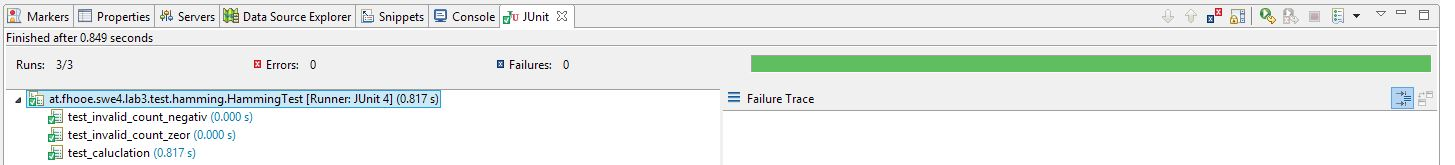
\includegraphics[width=\textwidth]{\imagesDir/tests_hamming_junit.JPG}
  \caption[JUnit Reulstat]
   {Diese Abbildung zeigt das Resultat der JUnit Tests im eclipse}
\end{figure}
\begin{figure}[h]
  \centering
  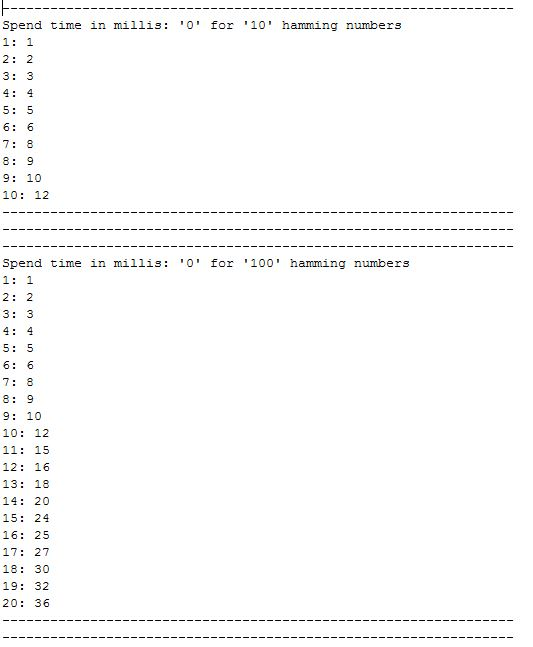
\includegraphics[scale=0.8]{\imagesDir/tests_hamming_console_1.JPG}
  \caption[Konsolenausgabe der Berechnungszeiten]
   {Diese Abbildung zeigt die Berechnungszeiten für 10 und 100 Hammingzahlen}
\end{figure}
\newpage
\begin{figure}[h]
  \centering
  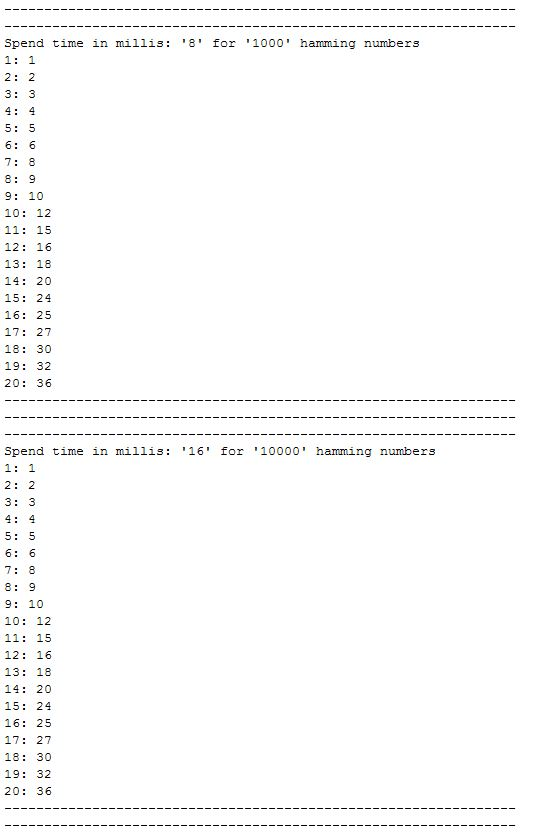
\includegraphics[scale=0.8]{\imagesDir/tests_hamming_console_2.JPG}
  \caption[Konsolenausgabe der Berechnungszeiten]
   {Diese Abbildung zeigt die Berechnungszeiten für 1000 und 10.000 Hammingzahlen}
\end{figure}
\newpage
\begin{figure}[h]
  \centering
 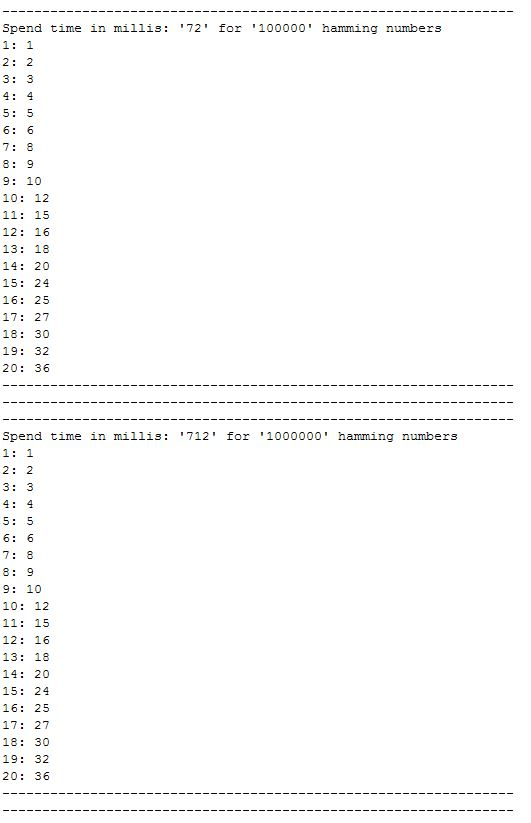
\includegraphics[scale=0.8]{\imagesDir/tests_hamming_console_3.JPG}
  \caption[Konsolenausgabe der Berechnungszeiten]
   {Diese Abbildung zeigt die Berechnungszeiten für 100.000 und 1.000.000 Hammingzahlen}
\end{figure}
% =============================================
% 2. Sorting algorithms
% =============================================
% Idea (common)
% =============================================
\newpage
{\color{myred}
	\section
		{Sortieralgorithmen}
}
\subsection{\ideaSection \hspace{2mm}(Allgemein)}
Folgend sind die Lösungsideen der Sortierlagorithmen HeapSorter und QuickSorter angeführt.\\
Da beide Algorithmen denselben output liefern sollen, soll hier ein Interface spezifiziert werden welches die Funktionalität bzw. die zu implementierenden Methoden Signaturen vorgibt. Die Aufgabenstellung verlangt zwar nur das Sortieren auf Integer Felder, jedoch sollen die Algorithmen so implementiert werden, dass sie auf Typen, die das Interface \inlinecode{Compareable<E>} implementieren. Daher muss das Interface folgende Signatur vorweisen.\inlinecode|public Sorter<E extends Comparable<E>> {...}|
\newpage
% =============================================
% Source (common)
% =============================================
\subsubsection{Source Code\hspace{2mm}{Allgemein}}
Folgend sind die allgemeinen Sources der Sortieralgorithmen angeführt.
\lstinputlisting[style=sourceFileStyle]{\mainPackage/sort/api/Sorter.java}
\newpage
% =============================================
% 2.1 Statistics
% =============================================
% Idea (stastistics)
% =============================================
\subsection{\ideaSection \hspace{2mm}(Statistics)}
Aufgrund dessen dass die Sortieralgorithmen mit Code Statistics versehen werden sollen, sollen Klassen implementiert werden, die es erlauben die verlangten Statistics zu ermitteln und auch einen Report dieser zu erstellen.\\
Hierbei soll diese Code Statistics wie folgt aufgeteilt werden:
\begin{enumerate}
	\item \textbf{StatisticsProvider:} Das Interface welches die Spezifikation für den Code Statistik Provider enthalten soll.\\
	Die Implementierung soll es ermöglichen mehrere Statistik Kontexte zu verwalten.
	\item \textbf{StatisticContext:} Die Klasse, welche einen Statistik Kontext darstellen soll.\\
	Dieser Kontext soll es ermöglichen mehrere CodeStatistic Instanzen pro Kontext zu verwalten.
	\item \textbf{CodeStatistic:} Die Klasse, die die Code Statistik Informationen (swap, compare counts) halten soll
	\item \textbf{DefaultStatisticProviderImpl:} Die default Implementierung des Interface StatisticProvider, welches die Funktionalitäten implementiert soll.
\end{enumerate}
Alle Klassen sollen die \inlinecode{instance.toString()}  Methode überschreiben und jeweils ihre beinhaltenden Informationen als \inlinecode{String} zurückliefern, wobei ein Parent bzw. die Klasse die Instanzen einer anderen verwaltet and deren \inlinecode{child.toString()} zu delegieren.
\newpage
% =============================================
% Idea (statistics)
% =============================================
\subsubsection{Source Code}
Folgend ist der Source der Statistik Implementierungen und Interfaces angeführt.
\lstinputlisting[style=sourceFileStyle]{\mainPackage/stat/api/StatisticsProvider.java}
\lstinputlisting[style=sourceFileStyle]{\mainPackage/stat/StatisticContext.java}
\lstinputlisting[style=sourceFileStyle]{\mainPackage/stat/CodeStatistics.java}
\lstinputlisting[style=sourceFileStyle]{\mainPackage/stat/DefaultStatisticsProviderImpl.java}

% =============================================
% 2.2 HeapSorter
% =============================================
% Idea (heapsorter)
% =============================================
\newpage
\subsection{HeapSorter}
Folgend ist die Lösungsidee für die HeapSorter Implementierung angeführt.\\
Da hierbei eine Heap Implementierung von Nöten ist und diese aber auch anderweitig verwendet werden könnte soll ein Heap Implementiert werden, der unabhängig von einem HeapSorter verwendet werden kann. Da wir auch hier generisch bleiben wollen und es auch möglich sein soll eine Heap Implementierung mit einem anderen Container zu implementieren (Bsp.: \inlinecode{ArrayList<E>}, \inlinecode{T[]}, usw.) soll ein Interface spezifiziert werden, welches die Funktionalitäten eines Heap spezifiziert. Es soll folgende Signatur haben
\inlinecode|public Heap<E extends Comparable<E>> {...}|\\
Des Weiteren soll eine Enumeration spezifiziert werden, die es erlaubt zu definieren, ob der Heap ein upheap oder downheap sein soll, also ob der root das höchste oder kleinste Element darstellt.\\\\
Ansonsten soll der Heap wie bekannt implementiert werden.
% =============================================
% Source(heapsorter)
% =============================================
\subsubsection{Source Code}
Folgend ist der Source der Interfaces und Implementierungen für Heap und Heap Sorter angeführt.
\lstinputlisting[style=sourceFileStyle]{\mainPackage/sort/api/Heap.java}
\lstinputlisting[style=sourceFileStyle]{\mainPackage/sort/heap/impl/HeapArrayListImpl.java}
\lstinputlisting[style=sourceFileStyle]{\mainPackage/sort/heap/impl/HeapSorter.java}
% =============================================
% Tests (heapsorter)
% =============================================
\newpage
\subsubsection{\testSection}
Folgend sind die Tests für die HeapSorter Implementierung angeführt.\\
Diese Tests können einfach in einem eclipse erneut ausgeführt und reproduziert werden, obwohl anzumerken ist, dass die Zeiten abhängig von den zu Verfügung stehenden Ressourcen abhängig sind.
\begin{figure}[h]
  \centering
  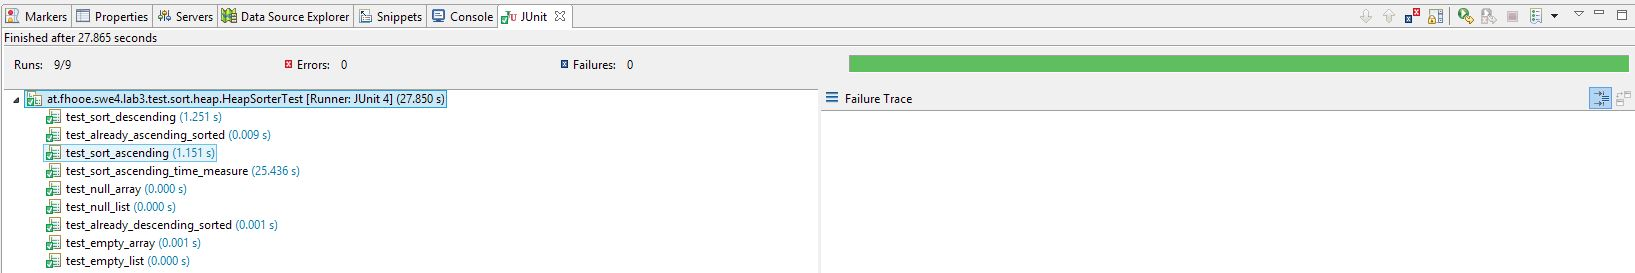
\includegraphics[width=\textwidth]{\imagesDir/tests_heap_junit.JPG}
  \caption[JUnit Resultat]
   {Diese Abbildung zeigt das Resultat der JUnit Tests in eclipse}
\end{figure}
\newpage
\begin{figure}[h]
  \centering
  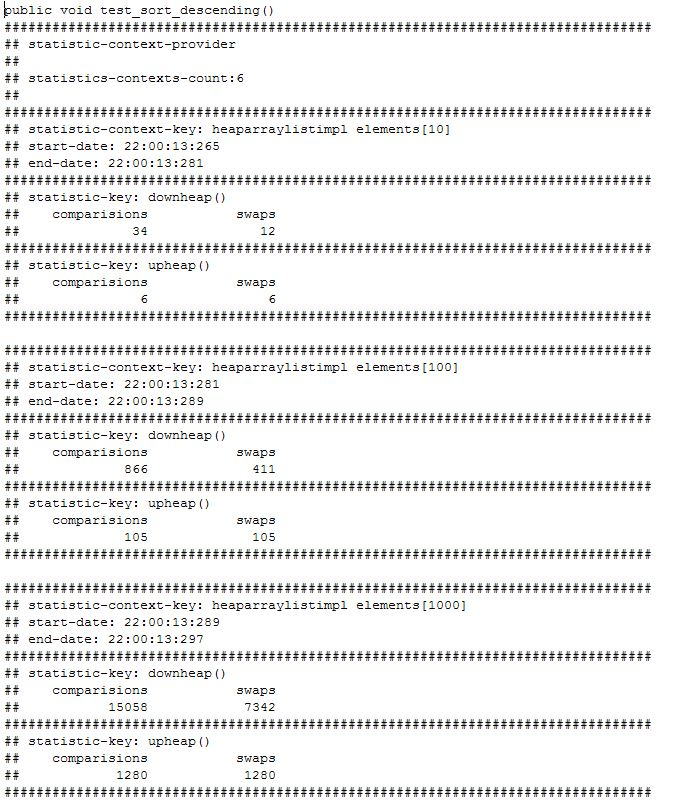
\includegraphics[scale=0.8]{\imagesDir/tests_heap_console_1.JPG}
  \caption[Konsolenausgabe der Statistiken]
   {Diese Abbildung zeigt die Statistiken für das Sortieren von 10, 100, 1.000 Elementen}
\end{figure}
\newpage
\begin{figure}[h]
  \centering
  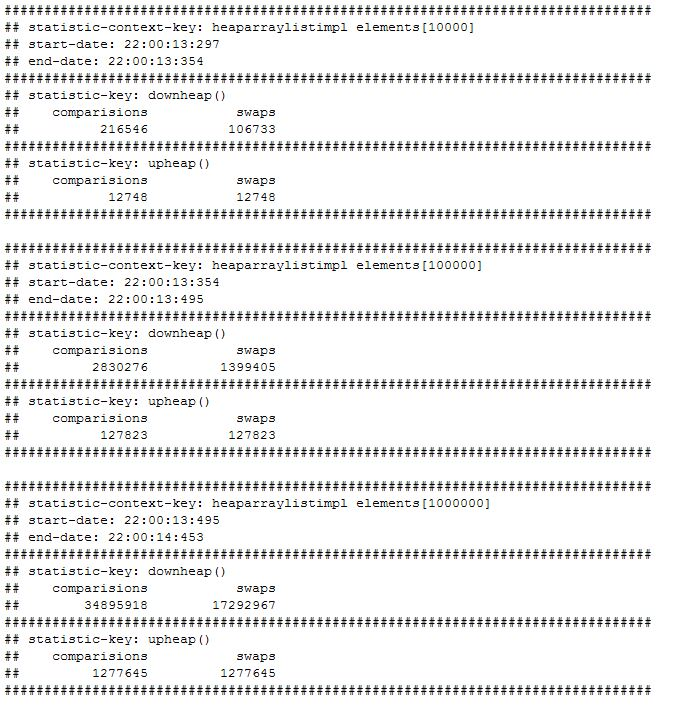
\includegraphics[scale=0.8]{\imagesDir/tests_heap_console_2.JPG}
  \caption[Konsolenausgabe der Statistiken]
   {Diese Abbildung zeigt die Statistiken für das Sortieren von 10.000, 100.000, 1.000.000 Elementen}
\end{figure}
\newpage
\begin{figure}[h]
  \centering
  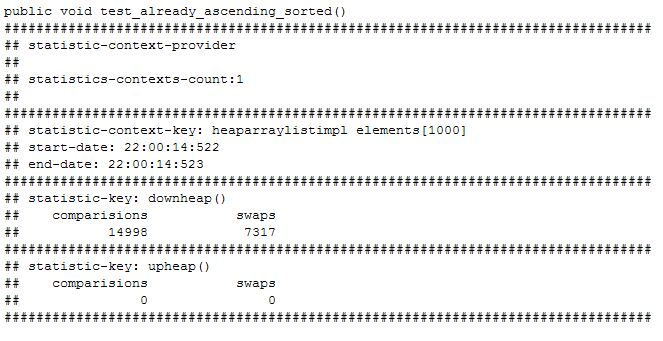
\includegraphics[scale=0.8]{\imagesDir/tests_heap_console_3.JPG}
  \caption[Konsolenausgabe der Statistiken]
   {Diese Abbildung zeigt die Statistiken für das Sortieren von 1.000 Elementen die bereits aufsteigend sortiert sind}
\end{figure}
\newpage
\begin{figure}[h]
  \centering
  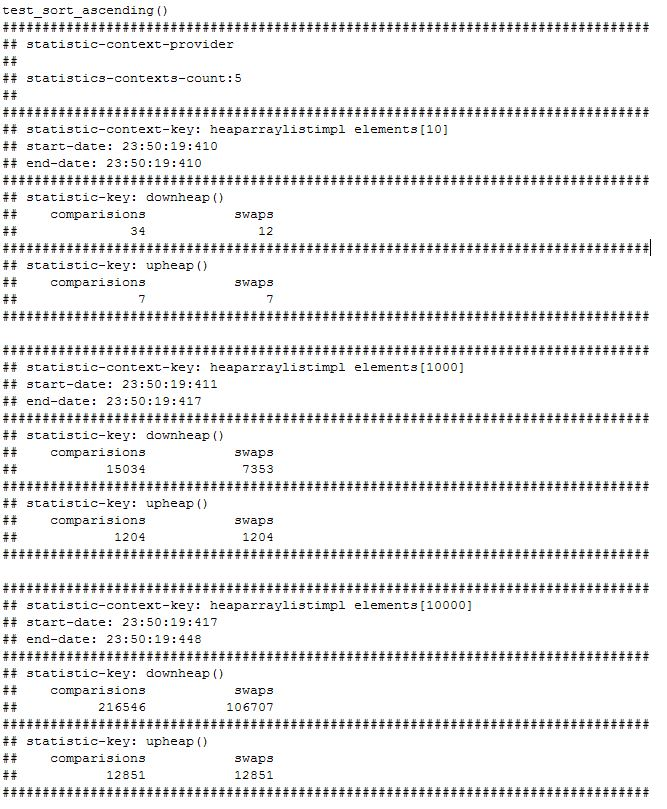
\includegraphics[scale=0.8]{\imagesDir/tests_heap_console_4.JPG}
  \caption[Konsolenausgabe der Statistiken]
   {Diese Abbildung zeigt die Statistiken für das Sortieren von 10, 100, 1.000 Elementen}
\end{figure}
\newpage
\begin{figure}[h]
  \centering
  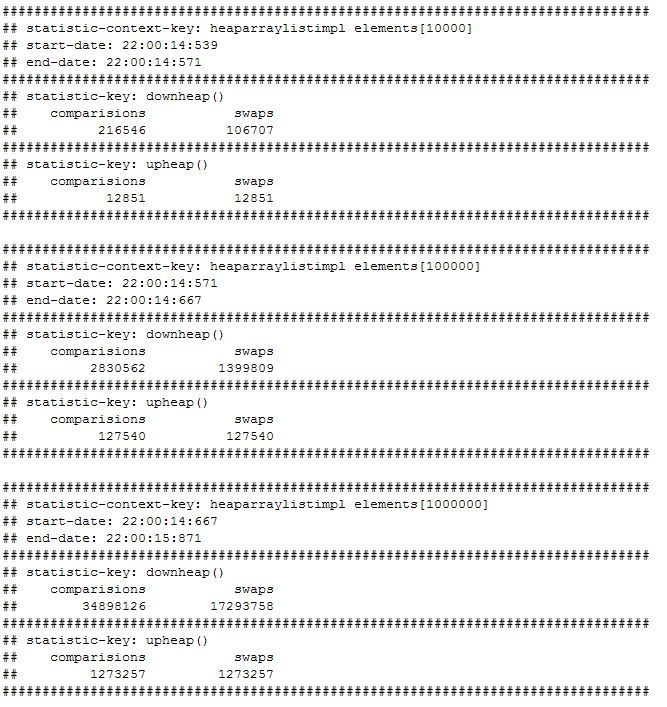
\includegraphics[scale=0.8]{\imagesDir/tests_heap_console_5.JPG}
  \caption[Konsolenausgabe der Statistiken]
   {Diese Abbildung zeigt die Statistiken für das Sortieren von 10.000, 100.000, 1.000.000 Elementen}
\end{figure}
\newpage
\begin{figure}[h]
  \centering
  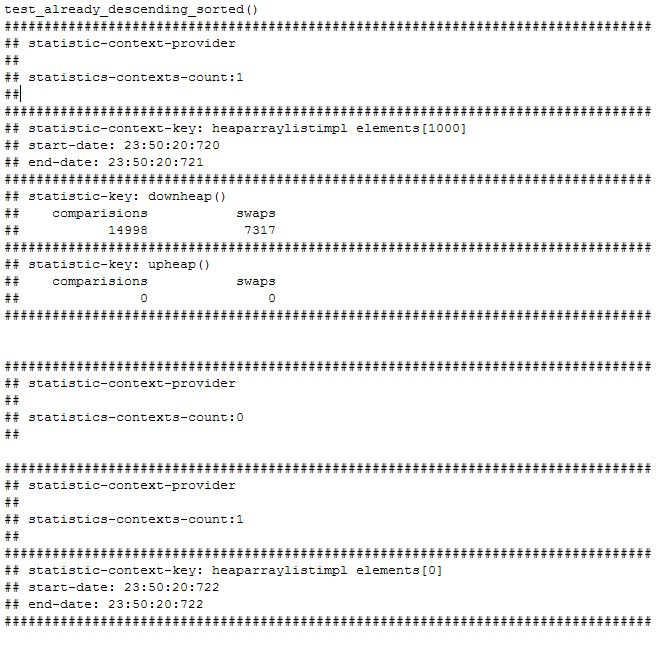
\includegraphics[scale=0.8]{\imagesDir/tests_heap_console_6.JPG}
  \caption[Konsolenausgabe der Statistiken]
   {Diese Abbildung zeigt die Statistiken für das Sortieren 1.000 Elementen die bereits absteigend sortiert sind}
\end{figure}
% =============================================
% 2.2 WucikSorter
% =============================================
% Idea (quicksorter)
% =============================================
\newpage
\subsection{QuickSorter}
Folgend ist die Dokumentation für den QuickSorter angeführt.\\
Diese Implementierung soll ebenfalls das Interface \inlinecode{Sorter<E>} implementieren und die CodeStatistics verwenden.\\
Entweder soll der Algorithmus so gewählt werden dass er aufsteigend und absteigend sortieren kann, oder die  Liste soll bei der inversen Sortierung mittels \inlinecode{Collections.reverse(list)} umgedreht werden.\\
Ansonsten ist der QuickSort Algorithmus wie bekannt zu implementieren.
% =============================================
% Source(quicksorter)
% =============================================
\subsubsection{Source Code}
Folgend ist der Source der QucikSort Implementierung angeführt.
\lstinputlisting[style=sourceFileStyle]{\mainPackage/sort/quick/QuickSorter.java}
% =============================================
% Tests (quicksorter)
% =============================================
\newpage
\subsubsection{\testSection}
Folgend sind die Test für die QuickSort Implementierung angeführt.
Diese Tests können einfach in einem eclipse erneut ausgeführt und reproduziert werden, obwohl anzumerken ist, dass die Zeiten abhängig von den zu Verfügung stehenden Ressourcen abhängig sind.
\end{document}  